The inducer is specific to the model. However, in common, an inducer tries to minimize the expected loss of the model it produces. The expected loss is a property of the model solving a task and depends on the performance measure $P$ defined for the task. As will be seen, the expected loss is difficult to determine directly but will help understand the metrics used in machine learning. \cite{bishop2006pattern}

This section is written based on \cite{bishop2006pattern} but emphasizes the difference between the objective truth $ot(.)$ and ground truth $gt(.)$ and uses the definitions provided in the last section. The exact formulas used can be found in \cite{bishop2006pattern}.

% ot -noise-> gt 
Let us assume a task $(\mathbb{I}, \mathbb{T}, ot(.))$. The data generation process will be the first step in producing a trained machine learning model to tackle the task. The process generates the dataset by sampling the objective truth $ot(.)$ via experiments (there is a data-generation distribution \cite{bengio2017deep}). Therefore the process abstracts from the objective truth $ot(.)$ to the ground truth $gt(.)$. As $gt(.)$ only refers to the samples taken it turns out to be a partial function $gt: \mathbb{I} \to \mathbb{T}$. In this work, the ground truth refers to the samples in the dataset and, therefore, it holds
\[(\mathbf{x}_i,t_i) \in D \Longleftrightarrow (\mathbf{x}_i \mapsto t_i) \in \mathcal{G}_{gt}\]

As random fluctuations might be involved in the experiments, the dataset can already contain errors known as noise.

% Generalization
Usually, only a restricted number of samples are available when the inducer creates the trained model. Nevertheless, the model should be able to approximate the objective truth $ot(.)$ as well as possible for all possible inputs in $\mathbb{I}$. The capability of transferring the knowledge seen to new inputs is called generalization. The generalization capabilities of the model are measured using a so-called train-test split. The train-test split splits up the dataset into two disjoint subsets $D_{\text{train}}$ and $D_{\text{test}}$. Then $D_{\text{train}}$ should be used to train the model and $D_{\text{test}}$ to approximate the capabilities of the model, to generalize using the performance measure $P$. 

Generalization can be further understood by decomposing the expected loss into the bias, the variance, and the noise. The origin of the noise is the sampling process, so the bias and the variance still need to be explained.

Both terms are defined with respect to a model trained on different datasets $D_1,D_2,\dots$ but for the same task. That is, an inducer $\mathcal{I_\zeta}$ creates the models via $M_{\theta_1} = \mathcal{I_\zeta}(D_1), M_{\theta_2} = \mathcal{I_\zeta}(D_2),\dots$. The bias is the extent to which the average prediction of the models deviates from the objective truth, and variance is the extent to which the models' predictions vary around the average prediction.
If the variance term dominates, that might imply that the model mainly learned the characteristics of the dataset used during training and, therefore, generalizes poorly to unseen data. On the other hand, if the bias term dominates, that might be a sign that the model is generally not capable of learning the needed structures or the inducer with the given hyperparameters can not learn the required model $M$ as $M \not\in \mathcal{F_{I_\zeta}}$. Therefore, a well-trained model usually needs a balanced bias and variance: The model is biased enough to generalize well but sufficiently complex to adopt the dataset's structure. 

The following example shows that in some cases approximating the expected loss of the model $M_\theta$ via $P$ on $D_{\text{test}}$ is enough. That is important as determining the concrete bias-variance decomposition often cannot be done as the required amount of data is unavailable and $ot(.)$ is not accessible. Furthermore, the example visualizes the concepts of bias, variance, noise, objective truth, and ground truth.

\begin{Bsp}{Estimating the required depth of a decision tree to approximate the sigmoid function}{sigmoid_estimation_example}
In this example, the sigmoid function $ot(x) = \frac{1}{1 + e^{-x}}$ should be approximated by regression. Here a decision tree for regression is used, but any other model used for regression could be used. Most important is that the inducer used to train the model needs to have a hyperparameter, which limits the complexity of the model. A study is done to find the maximum depth of the decision tree such that the model generalizes well. Following the procedure described to explain the bias and the variance for each possible depth, $100$ decision trees are trained on a dataset $D_j$ sampled from $ot(.)$. Each dataset has $N = 1000$ samples and is divided by a train-test split. During the process, for each depth, the average squared loss using a distinct test dataset is calculated:
\[
\frac{1}{100 * N} \sum_{j=1}^{100} \sum_{i=1}^N (M_{\theta_j}(\mathbf{x}_i) - t_i)^2
\]
This is done as the performance measure used here is the mean squared error.
The decision trees are used to estimate the bias, the variance, and the noise as the components of the expected loss. This decomposition and the average test error per depth are used to create Figure \ref{fig:example_bias_vs_variance}.

\captionsetup{type=htypei}
\begin{minipage}[t]{\linewidth}
            \centering
            \vspace{1ex}
            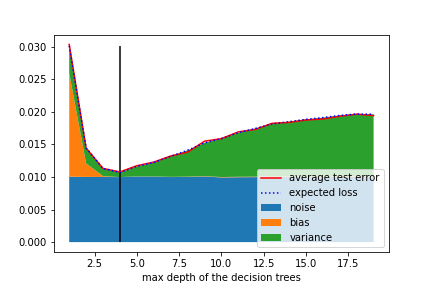
\includegraphics[width=9cm]{images/ml_basics/bias_variance_tradeoff.png}
            \captionof{figure}{Trading of bias vs. variance to estimate the maximal depth of a decision tree. Estimation is based on 100 decision trees trained on new sampled datasets with 1000 samples.}
            \label{fig:example_bias_vs_variance}
            \vspace{1ex}
\end{minipage}

First of all, one can see that the average test error strongly correlates with the expected loss. Although, the expected loss depends on $ot(.)$ and the average test error on $gt(.)$. To calculate the bias-variance decomposition from \cite{bishop2006pattern} $h(x)$, representing the optimal regression function is replaced by $ot(x)$.

The vertical line marks the depth of $4$, corresponding to the lowest expected loss and, therefore, the best possible value for the max depth hyperparameter. Next, the bias term dominates in the region of a too simple model, and the variance term dominates in the regions of a too complex model. Figure \ref{fig:example_bias_vs_variance_per_depth} visualize the model predictions per max depth and the bias-variance decomposition per input value. For example, in the Figure for a maximum depth of 8, one can see that the model has learned unnecessarily complex structures that only fit a particular dataset and, therefore, do not generalize well because of the high variance all over the place.  This is in contrast to a maximum depth of $1$, where the decision tree is incapable of capturing the structure of the sigmoid function, leading to a high bias term in large parts of the model.
Finally, the difference between the objective truth and the ground truth is visualized.
\captionsetup{type=htypei}
\begin{minipage}[t]{\linewidth}
    \centering
    \vspace{1ex}
    \begin{minipage}{\linewidth}
        \centering
        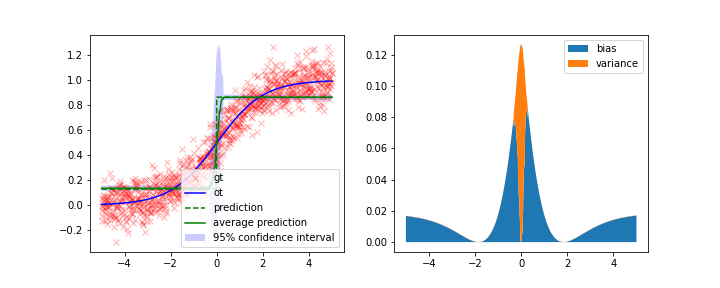
\includegraphics[width=12cm]{images/ml_basics/depth_1.png}\newline
        (a) max depth = 1
    \end{minipage}
    \vspace{0.3cm}
    \begin{minipage}{\linewidth}
        \centering
        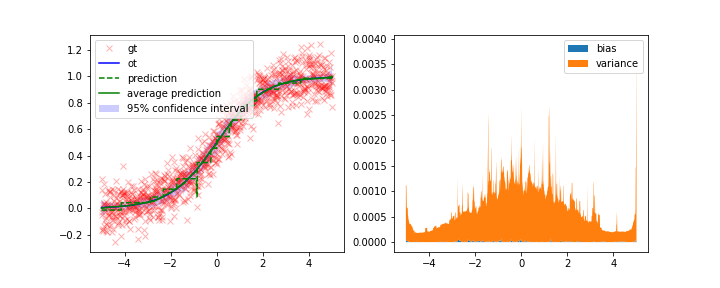
\includegraphics[width=12cm]{images/ml_basics/depth_4.png}\newline
        (b) max depth = 4
    \end{minipage}
    \vspace{0.3cm}
    \begin{minipage}{\linewidth}
        \centering
    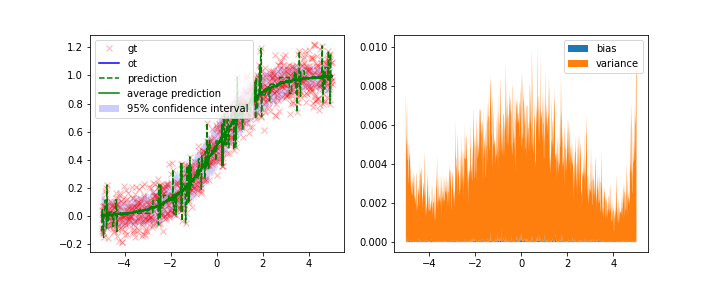
\includegraphics[width=12cm]{images/ml_basics/depth_8.png}\newline
        (c) max depth = 8
    \end{minipage}
    \captionof{figure}{Models' predictions and Bias-Variance Tradeoff visualized for a maximal depth of 1, 4 and 8. Refers to the experiment in Figure \ref{fig:example_bias_vs_variance}}
    \label{fig:example_bias_vs_variance_per_depth}
    \vspace{1ex}
\end{minipage}
\end{Bsp}

%Hence in a regression task the noise can be expressed as the mean squared error between the targets of $gt$ and $ot$ . Unfortunately most of the time this noise cannot be determined certainly as $ot$ can only be sampled. % To sum up the objective truth $ot$ gives the objectively correct answer while the ground truth $gt$ approximates the objective truth through samples.

%By doing so the predictive capabilities of the model with respect to $gt$ can be approximated, which therefore also approximates the capabilities of the model to generalize.

%As the objective truth is only available through samples in the ground truth, the performance of the model can only be measured against the ground truth. To do that 
